\documentclass[UTF8]{ctexart}
% 基本设置和必要宏包
\usepackage{geometry}
\geometry{a4paper,scale=0.8}

% 数学相关宏包
\usepackage{amsmath}
\usepackage{amssymb}
\usepackage{amsfonts}

\usepackage{mathtools}
\usepackage{amsbsy}
\usepackage{amstext}
\usepackage{wasysym}
\usepackage{stmaryrd}
\usepackage{mathrsfs}

% 图形和颜色
%\usepackage{xcolor}
\usepackage{graphicx}
\usepackage{subcaption}
\usepackage{caption}
\usepackage{float}


% 其他功能性宏包
\usepackage{titlesec}
\usepackage{fancyhdr}
\usepackage{setspace}
\usepackage{cite}
\usepackage{appendix}
\usepackage{listings}
\usepackage{pdfpages}
\usepackage{enumitem}
\usepackage{tabu}
\usepackage{threeparttable}
\usepackage{booktabs}
\usepackage{abstract}


\usepackage{diagbox} 
% 设置全局字体
%\setCJKmainfont{SimSun} % 设置正文为宋体
%\setCJKsansfont{SimHei} % 设置无衬线字体为黑体

% 允许公式跨页
\allowdisplaybreaks[4]



\newcommand{\sihaoheiti}{\fontsize{14pt}\selectfont\heiti}

% 论文题目设置为三号黑体字,并居中
\newcommand{\threelargebf}{\fontsize{16pt}{19.2pt}\selectfont\heiti\centering}

% 一级标题设置为四号黑体字,并居中
\titleformat{\section}{\centering\fontsize{14pt}{16pt}\bfseries\heiti}{\thesection}{1em}{}

% 二级标题设置为小四号黑体字,左对齐
\titleformat{\subsection}{\fontsize{12pt}{14.4pt}\bfseries\heiti}{\thesubsection}{1em}{\raggedright}

% 三级标题设置为小四号黑体字,左对齐
\titleformat{\subsubsection}{\fontsize{12pt}{14.4pt}\bfseries\heiti}{\thesubsubsection}{1em}{\raggedright}

% 正文字体设置为小四号宋体字,并使用单倍行距
\renewcommand{\normalsize}{\fontsize{12pt}{14.4pt}\selectfont}


%\linespread{5.0}%修改行距
% 图片文件夹
\graphicspath{{img/}}

\let\itemize\compactitem
\let\enditemize\endcompactitem

% 设置页面布局
\geometry{a4paper, left=2.5cm, right=2.5cm, top=3cm, bottom=3cm}
\setstretch{1.2}

\renewcommand{\arraystretch}{1.5}
\newcommand{\thickhline}{\noalign{\hrule height 1.2pt}} % 设置粗线的宽度
\newcommand{\thinhline}{\noalign{\hrule height 0.8pt}} % 设置细线的宽度

%%%% ===== 定理环境
\usepackage[amsmath,thref,thmmarks,hyperref]{ntheorem} % 定理宏包
%\theorempreskipamount1em % spacing before the environment
%\theorempostskipamount0em  % spacing after the environment
%\theoremstyle{plain}
%\theoremheaderfont{\normalfont\heiti}
%\theorembodyfont{\normalfont\kaishu}
%\theoremindent0em
%\theoremseparator{\hspace{0.2em}}
%\theoremnumbering{arabic}

\newtheorem{property}{性质}[section]
\newtheorem{definition}{定义}[section]
\newtheorem{lemma}{引理}[section]
\newtheorem{remark}{注记}[section]
\newtheorem{corollary}{推论}[section]
\newtheorem{example}{例}[section] 
\newtheorem{problem}{{问题}}

 \renewcommand{\abstractnamefont}{\normalfont\bfseries}  % 摘要标题字体:正常字体,粗体
\renewcommand{\abstracttextfont}{\normalfont\normalsize}     % 摘要内容字体:正常字体,小四号

% 设置页眉页脚
\pagestyle{fancy}
\fancyhf{}
\fancyfoot[C]{\thepage}
\renewcommand{\headrulewidth}{0pt}

% 设置标题格式
\titleformat{\section}{\centering\heiti\large}{\thesection}{1em}{}
\titleformat{\subsection}{\raggedright\heiti\normalsize}{\thesubsection}{1em}{}
\titleformat{\subsubsection}{\raggedright\heiti\normalsize}{\thesubsubsection}{1em}{}

% 设置摘要环境
%\newenvironment{myabstract}{
%	\begin{center}
%	\bfseries\zihao{-3} 摘要
%	\end{center}
%	\vspace{-0.5em} % 调整摘要与论文题目的距离
%	\normalsize
%}{
%}
% 设置附录环境
\renewcommand{\appendixname}{附录}
\renewcommand{\appendixpagename}{附录}

% 设置代码环境
\lstset{
	basicstyle=\small\ttfamily,
	keywordstyle=\color{blue},
	commentstyle=\color{green!70!black},
	stringstyle=\color{red},
	breaklines=true,
	numbers=left,
	numberstyle=\tiny,
	frame=tb,
	language=Python
}
\newcommand{\bbA}{\mathbb{A}}
\newcommand{\bbB}{\mathbb{B}}
\newcommand{\bbC}{\mathbb{C}}
\newcommand{\bbD}{\mathbb{D}}
\newcommand{\bbE}{\mathbb{E}}
\newcommand{\bbF}{\mathbb{F}}
\newcommand{\bbG}{\mathbb{G}}
\newcommand{\bbH}{\mathbb{H}}
\newcommand{\bbI}{\mathbb{I}}
\newcommand{\bbJ}{\mathbb{J}}
\newcommand{\bbK}{\mathbb{K}}
\newcommand{\bbL}{\mathbb{L}}
\newcommand{\bbM}{\mathbb{M}}
\newcommand{\bbN}{\mathbb{N}}
\newcommand{\bbO}{\mathbb{O}}
\newcommand{\bbP}{\mathbb{P}}
\newcommand{\bbQ}{\mathbb{Q}}
\newcommand{\bbR}{\mathbb{R}}
\newcommand{\bbS}{\mathbb{S}}
\newcommand{\bbT}{\mathbb{T}}
\newcommand{\bbU}{\mathbb{U}}
\newcommand{\bbV}{\mathbb{V}}
\newcommand{\bbW}{\mathbb{W}}
\newcommand{\bbX}{\mathbb{X}}
\newcommand{\bbY}{\mathbb{Y}}
\newcommand{\bbZ}{\mathbb{Z}}

\title{}
\author{}
\date{}

\begin{document}

\begin{titlepage}		
		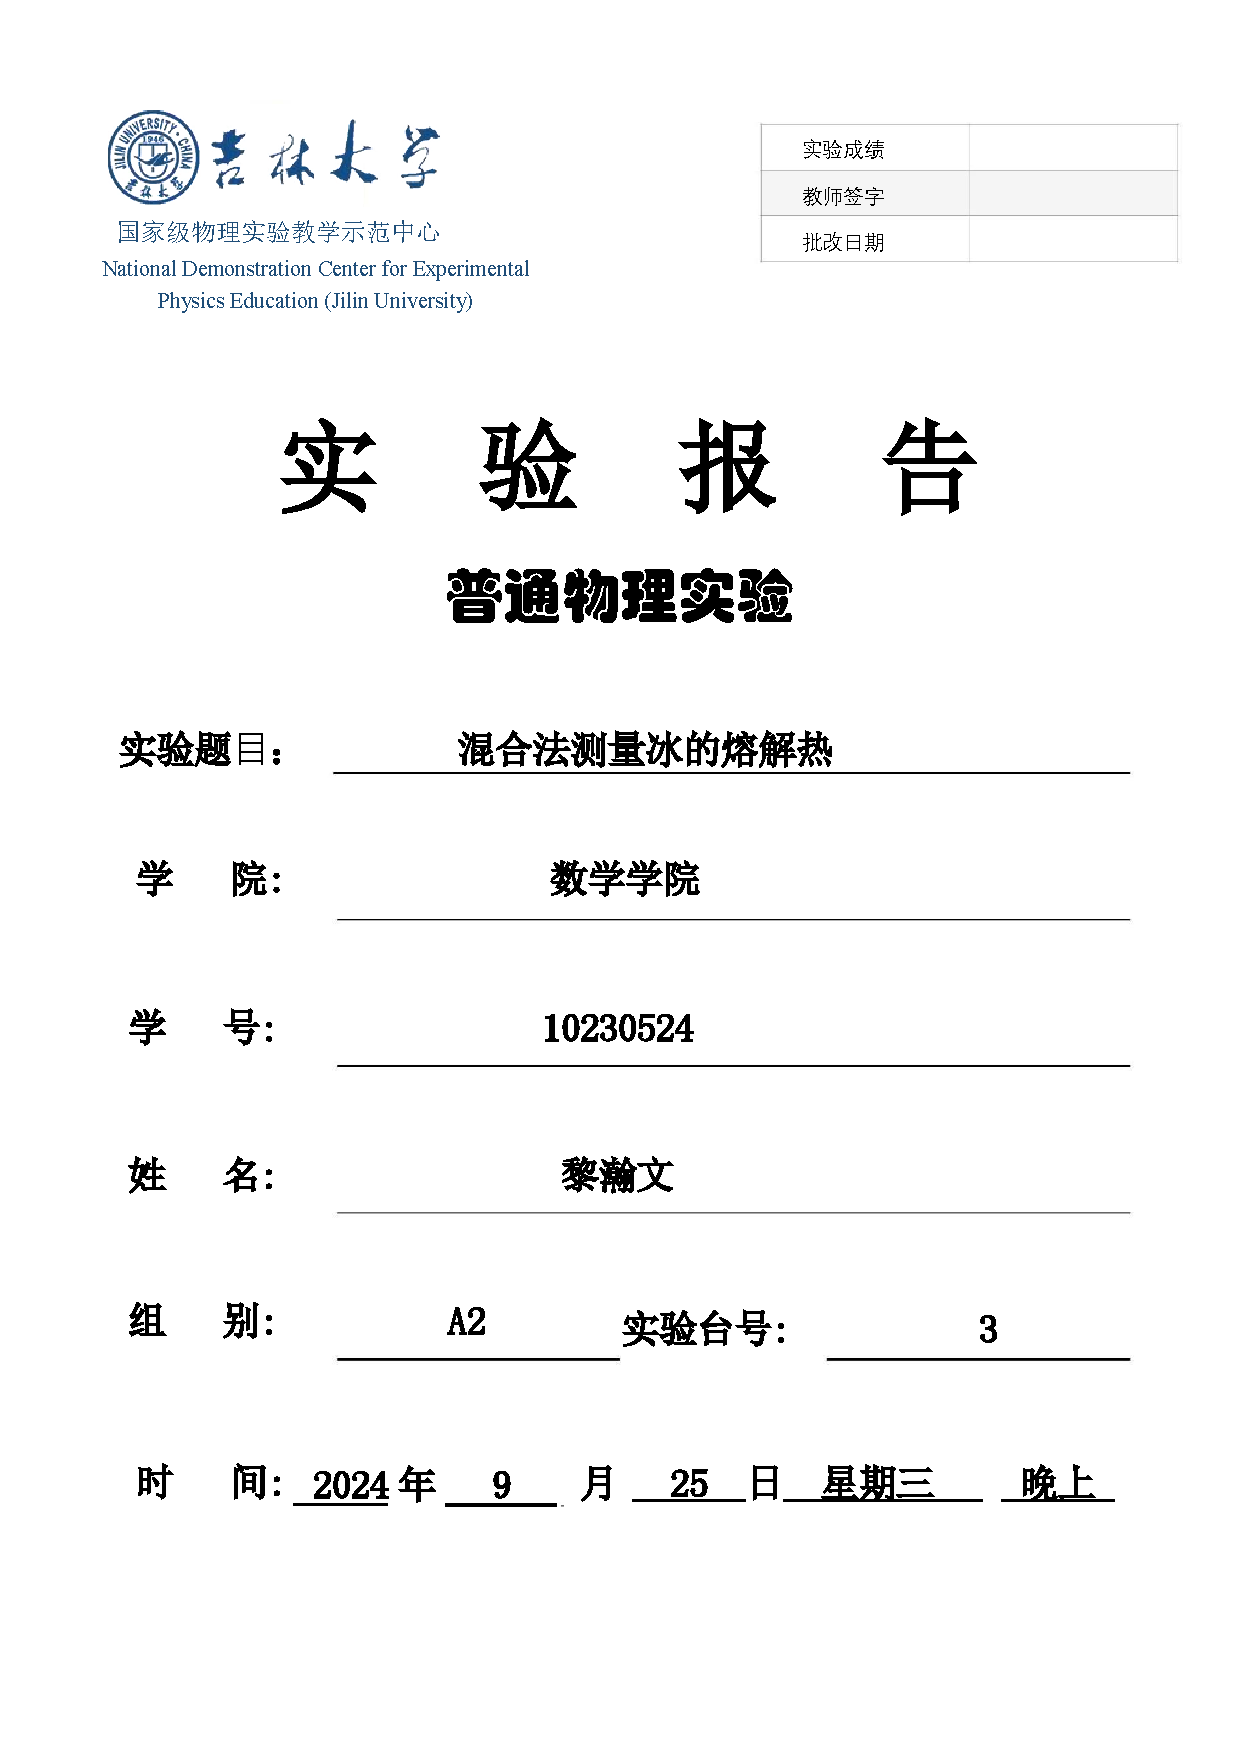
\includepdf[pages=-]{混合法封面.pdf}
\end{titlepage}


\section{实验内容}
\begin{enumerate}
    \item 擦干量热器内筒和搅拌器后称其质量$M_1$,并读出室温 $\theta$
    \item 将水盛到内筒总容积的 $\frac{1}{2}$ 处,加热至比室温高 $8 \pm 10^{\circ}C$
    \item 称量热器内筒、搅拌器和水的总质量$M_2$ 
    \item 取两块冰放在干毛巾上。放好内筒进入量热器,组装好温度计、搅拌器等后立即开始计时。每隔 $30s$ 记录一次温度计温度,同时不停搅拌并观察水温随时间的变化,共记录 $6$ 次共 $6$ 个点 
    \item 用干布擦干干冰表面的水,在不能溅起水花的前提下将冰迅速放入内筒水中;同时记录混合水系统初温 $T_1 \ ^{\circ}C$与时间,继续不停搅拌,每 $15s$ 记录一次温度,直至系统温度降至末温 $T_2 \ ^{\circ}C$
    \item 仍继续进行搅拌并观察水温随时间 $t$ 的变化,每隔 $30s$ 记录一次共记录 $5$ 次
    \item  将内筒取出称其质量,并计算水及冰的质量
\end{enumerate}

% 实验环境数据
\section{原始数据}

\begin{table}[H]
\centering
\caption{$1atm$下实验环境数据}
\begin{tabular}{|c|c|}
\hline
      温度 & $24^{\circ}C$ \\
\hline
      湿度 & $68\%$ \\
\hline
\end{tabular}
\end{table}


% 质量测量数据
\begin{table}[H]
\centering
\caption{质量的测量数据}
\begin{tabular}{|c|c|}
\hline
      内筒和搅拌器质量$m_1/g$ & 173.81 \\
\hline
      内筒、搅拌器和水的质量$2_2/g$ & 393.60 \\
\hline
      内筒、搅拌器、水和冰的质量 $3_3/g$ & 453.35 \\
\hline
\end{tabular}
\end{table}

% 仪器精确度测量数据
\begin{table}[H]
\centering
\caption{仪器精确度}
\begin{tabular}{|c|c|c|}
\hline
     & 电子天平 & 数字温度计 \\
\hline
     精确度 & 0.01g & $0.1^{\circ}C$ \\
\hline 
\end{tabular}
\end{table}

% 实验搅拌过程数据
\begin{table}[H]
\centering
\caption{记录搅拌数据}
\begin{tabular}{|c|c|c|c|c|c|c|c|c|}
\hline
    时间 & $0''$ & $30''$ & $1'$ & $1'30''$ &  $2'$ & $2'30''$  & $3'$  &   \\
\hline
    温度$^{\circ}C$ & 33.3 & 33.2 & 33.1 & 33.1 & 33.0  &  32.9 & 26.7  &    \\
\hline
    时间 & $3'30''$ & $3'45''$ & $4'$ &$4'15''$ &  $4'30''$ & $4'45''$  & $5'$ & $5'15''$  \\
\hline
    温度$^{\circ}C$ & 23.2 & 20.3 & 17.9 & 16.6 & 15.7  & 15.1  &  14.6   &14.1  \\
\hline
  时间  & $5'30''$ & $5'45''$ & $6'$ &  $6'15''$ & $6'30''$  & $6'45''$ & $7'$  & $7'15''$ \\
\hline
    温度$^{\circ}C$ & 13.8 & 13.4 & 13.1 & 12.7  & 12.4  &  12.1  &  11.9 & 11.7 \\
\hline
  时间  & $7'30''$ & $7'45''$ & $8'$ &  $8'15''$ & $8'30''$  & $8'45''$ & $9'$  & $9'15''$ \\
\hline
    温度$^{\circ}C$  & 11.6 & 11.5 & 11.3  & 11.1  &  11.1   & 11.1 & 11.0 & 11.0  \\
\hline
  时间  & $9'30''$ & $9'45''$ & $10'$ &  $10'15''$ & $10'30''$  & $10'45''$ & $11'$  & $11'15''$ \\
\hline
    温度$^{\circ}C$  & 10.9 & 10.9  & 10.9  & 10.9  & 10.9&10.9 & 10.9& 10.9   \\
\hline
  时间  & $11'30''$ & $11'45''$ &  &  &   & &  &  \\
\hline
    温度$^{\circ}C$  & 10.9 & 11.0 &   &  & & & &     \\
\hline
  时间  & $12'$ & $12'30''$ & $13'$ &  $13'30''$ & $14'$  & $14'30''$ &  &  \\
\hline
    温度$^{\circ}C$ & 11.0 & 11.0 & 11.1 & 11.1 & 11.2  & 11.3  &    &   \\
\hline
\end{tabular}
\end{table}


\section{数据处理与分析}
\subsection{作系统温度随时间变化曲线图并修正初温、末温}
\vspace{12cm} %5mm vertical space
% 实验课上老师会发坐标纸作图,然后粘贴到此处,根据书上或课上的方法作图


\vfill
由图解修正法得到修正后的系统初温 $T_1 = 32.5^{\circ} C$,系统末温$T_2 = 10.0^{\circ} C$

\subsection{冰的熔化热计算}
由实验室测量原始数据及图解修正得到的数据如下:

水的质量 $m'= 393.60g - 173.81g =  219.79g$ 

冰的质量 $m= 453.35g - 393.60g =  59.75g$ 

由图解修正法得到的系统初温  $T_1 = 32.5^{\circ} C$,系统末温$T_2 = 10.0^{\circ} C$

查阅资料得到 水的比热容为 $c = 4.181J/(g\    ^{\circ}C)$,假设量热器内筒和搅拌器的材质相同,得到量热器的内筒和搅拌器的比热容 $c_1 = 0.39J/(g\    ^{\circ}C)$

综合上述数据代入公式
\begin{align*}
    L =  \frac{m'c+m_1c_1}{m}(T_1 - T_2) - cT_2 
\end{align*}

得到 $L =  329.76 J/g$

\subsection{计算$L$的扩展不确定度}
\subsubsection{计算质量的不确定度}
由于量热器内筒和搅拌器质量$m_1$、以及其和水总质量 $m_2$、 其与水和冰的总质量 $m_3$ 均由电子天平测量得到,则它们的 $A$类测量不确定度 均假设为 0 

假设误差均匀分布,则其 $B$类不确定度
\begin{align*}
    u_{B}(m_1) = u_{B}(m_2) = u_{B}(m_3) = \frac{0.01}{\sqrt{3}}g = 0.00577g
\end{align*}

由合成标准不确定度 $u_C(i) = \sqrt{u_A(i)^2 + u_B(i)^2}$ 得到  $$u_C(m_1) = u_C(m_2) = u_C(m_3) = 0.00577g$$

已知水和冰的质量的计算公式如下:
\begin{align*}
    m' &= m_2 - m_1 \\
    m  &= m_3 - m_2 
\end{align*}

根据不确定度传递公式 $u_C(y)=\sqrt{\sum_{i=1}^{n}(\frac{\partial y}{\partial x_i})^2u_C(x_i)^2}$ 可得 
\begin{align*}
    u_C(m') &= \sqrt{u_C(m_2)^2 +u_C(m_1)^2} \\
    u_C(m)  &= \sqrt{u_C(m_3)^2 +u_C(m_2)^2}
\end{align*}

得到 $u_C(m') = 8.16 \times 10^{-3}g$、$u_C(m)= 8.16 \times 10^{-3}g$

\subsubsection{计算温度的不确定度}
由于系统初温  $T_1 = 32.5^{\circ} C$,系统末温$T_2 = 10.0^{\circ} C$ 均为由图解法修正过后的温度,均为由线性拟合得到的数据而非实验测得

由于作图取纵坐标温度 $T$ 最小分度为 $0.25^{\circ} C$,同时假设概率密度满足均匀分布,则其测量得到的 $A$类标准不确定度均为 0 ,同时得到
\begin{align*}
    u_C(T_1) =  u_C(T_2) = u_B(T_1) = u_B(T_2) = \frac{0.25^{\circ} C}{\sqrt{3}} = 0.144337^{\circ} C
\end{align*}
\subsubsection{计算比热容的不确定度}
在实验室室温、湿度不改变的情况下 假设比热容不变。故不考虑其不确定度

\subsubsection{计算合成标准不确定度}
根据不确定度传递公式,合成标准不确定度

\begin{align*}
    u_C(L) = \sqrt{\sum (\frac{\partial L}{\partial x_i})^2u_C(x_i)^2 } 
\end{align*}
\begin{align*}
    u_C(L)^2 = 
     \Big( \frac{c(T_1 - T_2)}{m}u_C(m') \Big)^2 + \Big( \frac{c_1(T_1 - T_2)}{m}u_C(m_1) \Big)^2 +  \Big( \frac{m'c+m_1c_1}{m^2}(T_1-T_2)u_C(m) \Big)^2\\ + \Big( \frac{m'c+m_1c_1}{m}u_C(T_1) \Big) ^2 + \Big(  \frac{m'c+m_1c_1 -cm}{m}u_C(T_2) \Big) ^2
\end{align*}

得到其合成标准不确定度 $u_C(L) = 1.19115 J/g$

取置信概率为 $p = 0.955$, $K_p = 2$,代入扩展不确定度计算公式
\begin{align*}
    U(L) &= K_p \times u_C(L)  \\
    &= 2 \times 1.19115J/g = 2.38230 J/g
\end{align*}

保留两位小数得到 $U(L) = 2.38 J/g $

\subsubsection{汇总表示}
由上分析可得 冰的熔化热 $L =  \pm $ 置信概率 $p= 0.955$,$K_p = 2$
综上所述得到冰的熔化热为 $329.76 \pm 2.38 J/g$

\begin{table}[H]
\centering
\caption*{测量数据}
\begin{tabular}{c|c|c|c|c|c|c}
\toprule[1pt]
\midrule
     计算指标 & $i$ & $u_A(i)$ & $u_B(i)$ & $u_C(i)$ & $U(i)$  & $i=\overline{i} \pm U(i)$ \\
\midrule
 $m_1$ & 173.81 & 0  & $5.7710^{-3}$ & $5.77 \times 10^{-3}$  & & \\
\midrule
 $m_2$ & 393.60 & 0  & $5.7710^{-3}$  & $5.77\times 10^{-3}$  & & \\
\midrule 
$m_3$ & 453.35& 0  &  $5.7710^{-3}$ &  $5.77 \times 10^{-3}$ & & \\
\midrule
 $m'$ & 219.79 &   &  & $8.16 \times 10^{-3}$ &  & \\
\midrule
 $m$ & 59.75 &  & & $8.16 \times 10^{-3}$ & & \\
\midrule
 $T_1$ & 32.5 &  & $0.144337$ &  $0.144337$ & & \\
\midrule
 $T_2$ & 10.0& &  $0.144337$ &  $0.144337$ &  & \\
\midrule
 $L$ & 329.76 &  & & $1.19115$  & $2.38$ & $329.76 \pm 2.38$ \\
\midrule
\bottomrule[1pt]
\end{tabular}
\end{table}

由于表格篇幅所限,上述计算以及结果单位未标出,故在此进行补充。质量$m_1$、$m_2$、$m_3$、$m'$、$m$及其对应指标的单位为 $g$,温度$T_1$、$T_2$及其对应指标的单位均为 $^{\circ}C$,冰的熔化热 $L$ 及其指标的单位为 $J/g$












\newpage
\section{思考题}
\subsection{物体传递热量的方式}
物体传递热量的方式共三种,分别是热传导、热对流以及热辐射

\subsection{本实验的“”热力学系统”组成}
\begin{enumerate}
    \item 本实验中的“热力学系统”由量热器内筒、搅拌器、温度计组成
    \item 外筒不参与热交换,故不属于上述热力学系统
\end{enumerate}

\subsection{讨论各方面对实验结果的影响并阐述原因}
\subsubsection{测 $T_2$ 前搅拌不均匀或没有搅拌}
由于温度计测量的是内筒中下部分水的温度,若不搅拌会导致测量出的温度$T_2$ 偏高,从而使计算出的 $L$ 偏低
\subsubsection{测 $T_1$ 后没有很快放入冰,而是隔了一段时间}
$T_2$ 的测量修正了系统误差,故若图像绘制正确,得到的 $T_2$ 数据偏差不大或无影响,故对实验结果影响不大
\subsubsection{搅拌过程中水溅到了量热器的盖子上}
冰融化吸热,溅出的水不在内筒水中,故不会带走热量,导致整体溶剂减少,从而导致冰在吸热过程中测得的 $T_2$ 的值偏小,造成 $L$ 偏大

\subsubsection{冰中含水或冰上有没有擦干的水}
冰上有水会使需要融化冰的热量减少,从而使 $L$ 偏小

\subsection{确定实验室结露温度}
\begin{enumerate}
    \item 读取实验室温度和相对湿度,温度为 $24 ^{\circ}C$,相对湿度为 $68\%$ 
    \item 根据温度查水的饱和蒸汽压表,得到该温度下水的饱和蒸汽压值为 $2.9850kPa$
    \item 用所查得的温度下的水的饱和蒸汽压乘以相对湿度,得到空气中水汽的分压 $2.0298kPa$
    \item 根据空气中水汽分压差水的饱和蒸汽压表,该分压对应的温度为露点 $17.73 ^{\circ}C$
    \item 综上得到实验室的结露温度为 $17.73^{\circ}C$
\end{enumerate}
\end{document}